% Auriga theme
% find the most up-to-date version here: https://github.com/anishathalye/auriga

\documentclass[14pt,aspectratio=169]{beamer}
\usepackage{pgfpages}
\usepackage{fancyvrb}
\usepackage{tikz}
\usepackage{pgfplots}

\usepackage{amssymb}
\usepackage{relsize}
\usepackage{lipsum}
% \usepackage{tikz}
\usetikzlibrary{tikzmark, positioning, arrows.meta}
\usetikzlibrary{calc}

% \ifnotes
% \setbeamertemplate{note page}[plain]
% \setbeameroption{show notes on second screen=right}
% \fi

\usetheme{auriga}
\usecolortheme{auriga}

% define some colors for a consistent theme across slides
\definecolor{red}{RGB}{181, 23, 0}
\definecolor{blue}{RGB}{0, 118, 186}
\definecolor{gray}{RGB}{146, 146, 146}

\setbeamerfont{title}{size*={2pt}}
\title{\small Financialization of the Housing Market: A Contribution to Modern Urban Rent Theory}
    
% \author{Kirsten Wright} %\underline{Alyssa P. Hacker} \inst{1} \and Ben Bitdiddle \inst{2} \and Lem E. Tweakit \inst{2}}
\author{
  Author: Kirsten Wright \\
  Supervisors: Jangho Yang, Sean Geobey
}
% \institute{PhD Thesis Defensae}
\institute{PhD Thesis Defense\\[1ex] University of Waterloo}
\date{October 10, 2023}
% \institute[shortinst]{University of Waterloo} %{\inst{1} Some Institute \samelineand \inst{2} Another Institute}


% \title{Financialization of the Housing Market: A Contribution to Modern Urban Rent Theory}

% \author{Kirsten Wright}
% \subtitle{PhD Thesis Defense}
% \institute{University of Waterloo}
% \date{October 10, 2023}

\begin{document}

{
  % rather than use the frame options [noframenumbering,plain], we make the
  % color match, so that the indicated page numbers match PDF page numbers
  \setbeamercolor{page number in head/foot}{fg=background canvas.bg}
  \begin{frame}
    \titlepage
   % \vspace{1cm}
    \begin{center}
    \includegraphics[width=0.3\textwidth]{fig/uw.png}
    \end{center}
  \end{frame}
}


\begin{frame}
\begin{figure}[!ht]
\centering
% \hspace*{1cm} % Add 1cm of space to the left
\scalebox{0.5}{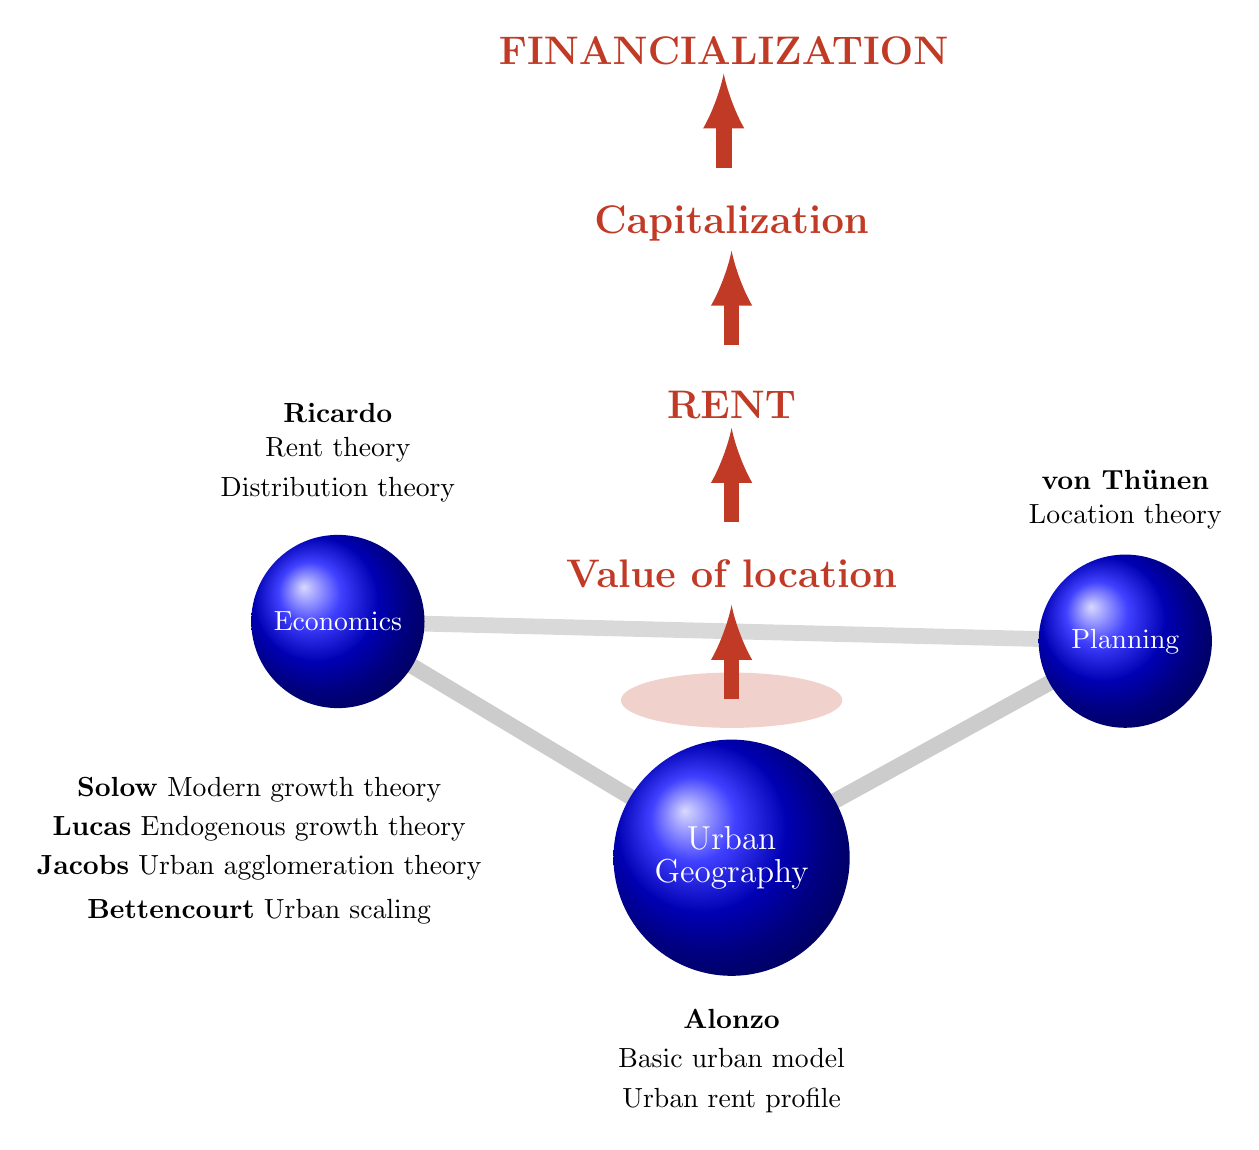
\begin{tikzpicture}{scale=.5}
% Find color for ball. Stop line short of node
\coordinate (planning) at (5,.75); % Preface
\coordinate (economics) at (-5,1); 
\coordinate (Ricardo) at (-5,1.4);
\coordinate (Solow) at (-6,1.25);
\coordinate (geography) at (0,-2); % History
\coordinate (finance) at (0,5); 

\draw [line width=2mm, black!15, ] (planning)--(economics);
\draw [line width=2mm, black!20, ] (geography)--(economics);
\draw [line width=2mm, black!20, ] (geography)--(planning);
%\draw [line width=2mm, black!25, ] (geography)--(finance);
%\draw [line width=2mm, black!20, ] (planning)--(finance);
%\draw [line width=2mm, black!20, ] (finance)--(economics);
%color=black!60!red
%\shade [ball color=blue!70] (5,5) circle (1.1cm)node[white] {\textbf{Planning}};
 
\node [circle,shading=ball,  minimum width=2.2cm, white, align=center] (ball) at (planning) {Planning};
\node [circle, shading=ball, minimum width=2.2cm, white, align=center] (ball) at (economics) {Economics};
\node [circle,shading=ball, minimum width=3cm, white, align=center] (ball) at (geography)[text width=2cm] {\large Urban \\ Geography};
%\node [circle, shading=ball, minimum width=2.4cm, white, align=center] (ball) at (finance)[text width=2cm] {Finance};
%\node at (-.3,-.1) [red] {\Large \textbf{RENT}};

\node at (planning) [above=1.8cm] {\textbf{von Th\"unen}};
\node at (planning) [above=1.3cm] {Location theory};

\node at (Ricardo) [above=2cm,]   {\textbf{Ricardo}};
\node at (Ricardo) [above=1.5cm] {Rent theory};
\node at (Ricardo) [above=1.0cm] {Distribution theory};

% \node at (Solow) [below=1.6cm, align=left] {\textbf{Solow:}};
\node at (Solow) [below=2.1cm, align=left] {\textbf{Solow} Modern growth theory};
\node at (Solow) [below=2.6cm, align=left] {\textbf{Lucas} Endogenous growth theory};
\node at (Solow) [below=3.1cm, align=left] {\textbf{Jacobs} Urban agglomeration theory};
\node at (Solow) [below=3.65cm, align=left] {\textbf{Bettencourt} Urban scaling};

\node at (geography) [below=1.8cm] {\textbf{Alonzo}};
\node at (geography) [below=2.3cm] {Basic urban model};
\node at (geography) [below=2.8cm] {Urban rent profile};
%\node [circle, shading=ball, minimum width=2.4cm, white, align=center] (ball) at (finance)[text width=2cm] {Finance};

\fill[red!20] (0,0) ellipse (40pt and 10pt);
%\node[red]at (1.2,0) {\large SPACE};
\begin{scope}[shift={(0,-.34)}]
\draw [line width=2mm, red!85, -latex ] (-.1, 7.1)--++(0,1.2)node[above=-.1] {\Large \textbf{FINANCIALIZATION}};
\draw [line width=2mm, red!85, -latex ] (0, 4.85)--++(0,1.2)node[above=-.1] {\Large \textbf{Capitalization}};
\draw [line width=2mm, red!85, -latex ] (0, 2.6)--++(0,1.2)node[above=-.1] {\Large \textbf{RENT}};
\draw [line width=2mm, red!85, -latex ] (0, .35)--++(0,1.2)node[above] {\Large \textbf{Value of location}};
%\draw [line width=2mm, red!85, -latex ] (0, -2)--++(0,-.8)node[above=-.1]  {\Large \textbf{SPACE}};
\end{scope}
\end{tikzpicture}}
\hspace*{1cm} % Add 1cm of space to the right
\end{figure}
\end{frame}

% Linking space and urban rents to the effects of financialization.]{Space and urban rents play a foundational role in urban economics, geography, and planning. We extend the analysis of urban rents to model the effects of financialization.
\input{slide_deck/slides/fig2}
% \input{slides/examples/bullets}
% \input{slides/examples/splitfigs}
% \begin{frame}
\[
\tikzmarknode{A}{f}(\tikzmarknode{B}{5}) = \tikzmarknode{C}{25}
\begin{tikzpicture}[overlay, remember picture,shorten <=1mm,
                    nodes={inner sep=1pt, align=center, font=\footnotesize}]
\draw (A.south) -- ++ (-1,-1) node[below] {The\\ machine};
\draw (B.south) -- ++ (.2,-1) node[below] {When\\ given 5};
\draw (C.south) -- ++ (.8,-1) node[below] {Gives\\ us 25};
\end{tikzpicture}
\vspace{3ex}
\]
\end{frame}

\begin{frame}
\[
\tikzmarknode{A}{f}(\tikzmarknode{B}{5}) = \tikzmarknode{C}{25}
\begin{tikzpicture}[overlay, remember picture,shorten <=1mm,
                    nodes={inner sep=1pt, align=center, font=\footnotesize},
                    every path/.style = {draw=red, Stealth-}] % <---
\draw (A.south) -- ++ (-1,-1) node[below] {The\\ machine};
\draw (B.south) -- ++ (.2,-1) node[below] {When\\ given 5};
\draw (C.south) -- ++ (.8,-1) node[below] {Gives\\ us 25};
\end{tikzpicture}
\vspace{3ex}
\]
\end{frame}


\begin{frame}{A slide with centered equation and explanation}
  \begin{center}
    \begingroup\larger[4]
    \[
    \tikzmarknode{n1}{\rho\frac{D\vec V}{Dt}}~=~\tikzmarknode{n2}{-\nabla p}
    + \tikzmarknode{n3}{\rho\vec g}+\tikzmarknode{n4}{\mu\nabla^2\vec V}
    \]
    \endgroup
  \end{center}
  
  \vspace{1ex}
  
  \begin{center}
    \begin{tikzpicture}[remember picture,shorten <=1mm,font=\footnotesize\sffamily]
      % Your TikZ code for the explanation here
    \end{tikzpicture}
  \end{center}
\end{frame}


\begin{frame}
\[\int\limits
  _{\tikzmarknode{a}{a}}
  ^{\tikzmarknode{b}{b}}\tikzmarknode{f}{f}(\tikzmarknode{x1}{x})
  \,\tikzmarknode{d}{\mathrm{d}}\tikzmarknode{x2}{x}
\begin{tikzpicture}[overlay,remember picture,cyan,>=stealth,shorten
 <=0.2ex,nodes={font=\tiny,align=left,inner ysep=1pt},<-]
  \draw ([xshift=-0.3ex]b.west|-x2) -- ++ (-1.5em,0) node[left] (l) {\textbf{Integral}};
  \draw (a.south) -- ++ (0,-1.5em) node[anchor=north west,align=left,xshift=-1.2ex]
    (u) {\textbf{Untergrenze}\\ Untere integrationsgrenze};
  \draw (b.north) -- ++ (0,1.5em) node[anchor=south west,align=left,xshift=-1.2ex]
    (o) {\textbf{Obergrenze}\\ Obere integrationsgrenze};
  \path (x1.north) ++ (0,1.5em) node[anchor=south west,xshift=-1.2ex] (il)
    {\textbf{Integrand}\\ Funktion \"uber die integriert werden soll};
  \draw (x1.north) |- ([xshift=0.3ex]il.south east);
  \path (d.south) ++ (0,-1.5em) node[anchor=north west] (diff)
    {\textbf{Differtential}};
  \draw (d.south) |- ([xshift=0.3ex]diff.south east);
  \draw ([xshift=0.3ex]x2.east) -- ++ (1.5em,0) node[right]  (r)
   {\textbf{Integrationsvariable}\\ Der Integrand wird \"uber $x$ integriert};
  \path let \p1=($(o.north)-(u.south)$),\p2=($(r.east)-(x2.east)$),
   \p3=($(a.west)-(l.west)$),\n1={\x2-\x3} in 
  \pgfextra{\xdef\tmpvspace{\y1}\xdef\tmphspace{\n1}};
\end{tikzpicture}\vcenter{\vspace{\tmpvspace}}
\hspace{\tmphspace} 
\]
\end{frame}



\begin{frame}{A slide with centered equation and annotations}
  \begin{center}
    \begin{relsize}{4}
    \begin{align*}
    \tikzmarknode{n1}{\rho\frac{D\vec V}{Dt}} &= \tikzmarknode{n2}{-\nabla p}
    + \tikzmarknode{n3}{\rho\vec g}+\tikzmarknode{n4}{\mu\nabla^2\vec V} \\
    \text{Total derivative} &= \text{Pressure gradient} + \text{Body force term} + \text{Diffusion term}
    \end{align*}
    \end{relsize}
  \end{center}
  
  \vspace{1ex}
  
  \begin{center}
    \begin{tikzpicture}[remember picture,shorten <=1mm,font=\footnotesize\sffamily]
      % Your TikZ code for the explanation here
    \end{tikzpicture}
  \end{center}
\end{frame}

\begin{frame}{Equation and Annotations}
  \begin{center}
    \begin{relsize}{4}
    \begin{align*}
    \tikzmarknode{n1}{\rho\frac{D\vec V}{Dt}} &= \tikzmarknode{n2}{-\nabla p}
    + \tikzmarknode{n3}{\rho\vec g}+\tikzmarknode{n4}{\mu\nabla^2\vec V} \\
    \text{Total derivative} &= \text{Pressure gradient} + \text{Body force term} + \text{Diffusion term}
    \end{align*}
    \end{relsize}
  \end{center}
  
  \vspace{1ex}
  
  \begin{center}
    \begin{tikzpicture}[remember picture,shorten <=1mm,font=\footnotesize\sffamily]
      % Your TikZ code for the explanation here
      \begin{scope}[nodes={text width=6.5em,align=left},node distance=1ex]
        \node (e1) {\underline{Total derivative}};
        \node[right=of e1.north east,anchor=north west] (e2) {\underline{Pressure gradient}\\[1em]
          Fluid flows in the direction\dots};
        \node[right=of e2.north east,anchor=north west] (e3) {\underline{Body force term}\\[1em]
          External forces\dots};
        \node[right=of e3.north east,anchor=north west] (e4) {\underline{Diffusion term}\\[1em]
          For a Newtonian fluid\dots};
      \end{scope}     
      \node[below=0.5ex of e1.south] (eq){$=$};
      \node[below=0.5ex of eq] (tot) {$\rho\left[\frac{\partial \vec V}{\partial t}
      +\left(\vec V\cdot\vec\nabla\right)\vec V\right]$};
      \path (tot.south west) -- (tot.south east) coordinate[pos=0.25] (tot1)
        coordinate[pos=0.75] (tot2);
      \node[below left=2ex and 0ex of tot.south,text width=4em,align=left] (c1) 
          {Change of velocity};
      \node[below right=2ex and 0ex of tot.south,text width=4em,align=left] (c2) {Convective term};
      \draw[cyan,-stealth] (c1) -- (tot1);
      \draw[cyan,-stealth] (c2) -- (tot2);
      \begin{scope}[overlay]
      \foreach \X in {1,...,4}
      {\draw[cyan,-stealth] (e\X) -- (n\X);} 
      \end{scope}
    \end{tikzpicture}
    \end{center}
\end{frame}



\begin{frame}{Equation and Annotations}
  \begin{center}
    \begin{relsize}{2} % Adjust the scaling factor as needed
    \begin{align*}
    \tikzmarknode{n1}{\rho\frac{D\vec V}{Dt}} &= \tikzmarknode{n2}{-\nabla p}
    + \tikzmarknode{n3}{\rho\vec g}+\tikzmarknode{n4}{\mu\nabla^2\vec V} \\
    \text{Total derivative} &= \text{Pressure gradient} + \text{Body force term} + \text{Diffusion term}
    \end{align*}
    \end{relsize}
  \end{center}
  
  \vspace{1ex}
  
  \begin{center}
    \begin{tikzpicture}[remember picture, shorten <=1mm, font=\small\sffamily] % Adjust font size here
      % Your TikZ code for the explanation here
      \begin{scope}[nodes={text width=6.5em,align=left},node distance=1ex]
        \node (e1) {\underline{Total derivative}};
        \node[right=of e1.north east,anchor=north west] (e2) {\underline{Pressure gradient}\\[1em]
          Fluid flows in the direction\dots};
        \node[right=of e2.north east,anchor=north west] (e3) {\underline{Body force term}\\[1em]
          External forces\dots};
        \node[right=of e3.north east,anchor=north west] (e4) {\underline{Diffusion term}\\[1em]
          For a Newtonian fluid\dots};
      \end{scope}     
      \node[below=0.5ex of e1.south] (eq){$=$};
      \node[below=0.5ex of eq] (tot) {$\rho\left[\frac{\partial \vec V}{\partial t}
      +\left(\vec V\cdot\vec\nabla\right)\vec V\right]$};
      \path (tot.south west) -- (tot.south east) coordinate[pos=0.25] (tot1)
        coordinate[pos=0.75] (tot2);
      \node[below left=2ex and 0ex of tot.south,text width=4em,align=left] (c1) 
          {Change of velocity};
      \node[below right=2ex and 0ex of tot.south,text width=4em,align=left] (c2) {Convective term};
      \draw[cyan,-stealth] (c1) -- (tot1);
      \draw[cyan,-stealth] (c2) -- (tot2);
      \begin{scope}[overlay]
      \foreach \X in {1,...,4}
      {\draw[cyan,-stealth] (e\X) -- (n\X);} 
      \end{scope}
    \end{tikzpicture}
    \end{center}
\end{frame}


% \input{slides/examples/split}
% \input{slides/examples/figure}
% \input{slides/examples/centered}
% \input{slides/examples/monospace}
% \input{slides/examples/brackets}
% \input{slides/examples/link}

\end{document}
